%!TEX root = ./fuzzylite-1.01.tex
\chapter*{Appendix}
\addcontentsline{toc}{chapter}{Appendix}
\section*{GUI Setup}
\addcontentsline{toc}{section}{GUI Setup}
	The following figure shows the Setup part of the GUI build for \fl.\\
	\vfill
\noindent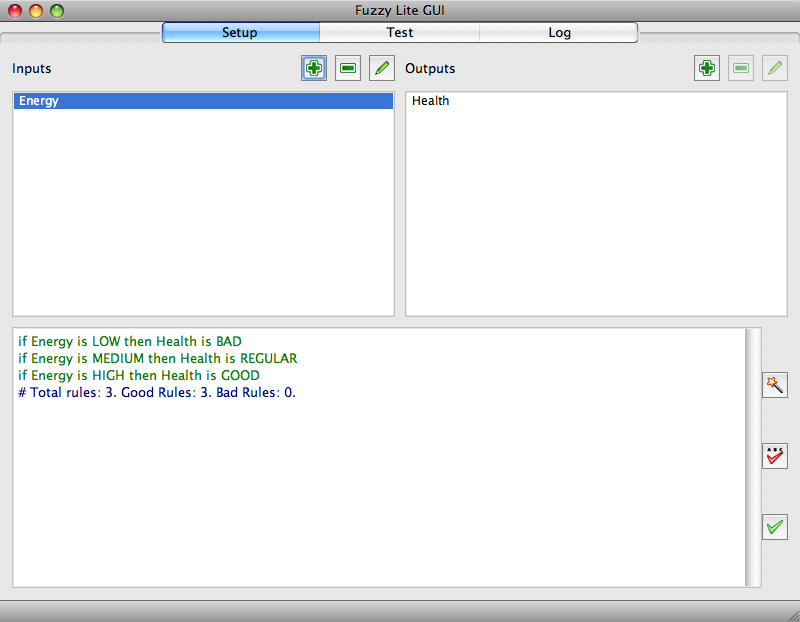
\includegraphics[scale=0.6]{./figures/gui-setup.png}
	\vfill

\clearpage
\section*{GUI Setup}
\addcontentsline{toc}{section}{GUI Test}
	The following figure shows the Setup part of the GUI build for \fl.\\
	\vfill
\noindent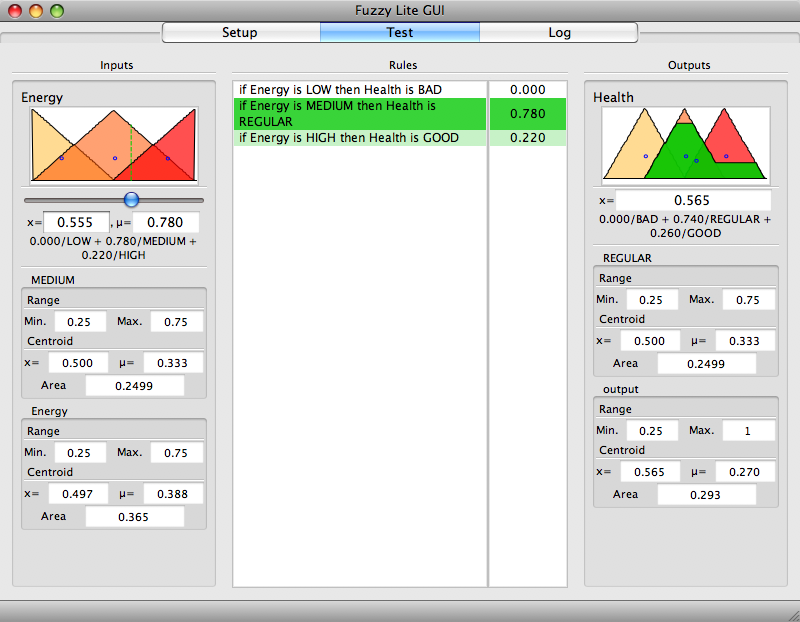
\includegraphics[scale=0.6]{./figures/gui-test.png}
	\vfill

\clearpage
\section*{License of \fl}
\addcontentsline{toc}{section}{License of \fl}
\begin{verbatim}
                             Apache License
                       Version 2.0, January 2004
                    http://www.apache.org/licenses/

TERMS AND CONDITIONS FOR USE, REPRODUCTION, AND DISTRIBUTION

1. Definitions.

  "License" shall mean the terms and conditions for use, reproduction,
  and distribution as defined by Sections 1 through 9 of this document.

  "Licensor" shall mean the copyright owner or entity authorized by
  the copyright owner that is granting the License.

  "Legal Entity" shall mean the union of the acting entity and all
  other entities that control, are controlled by, or are under common
  control with that entity. For the purposes of this definition,
  "control" means (i) the power, direct or indirect, to cause the
  direction or management of such entity, whether by contract or
  otherwise, or (ii) ownership of fifty percent (50%) or more of the
  outstanding shares, or (iii) beneficial ownership of such entity.

  "You" (or "Your") shall mean an individual or Legal Entity
  exercising permissions granted by this License.

  "Source" form shall mean the preferred form for making modifications,
  including but not limited to software source code, documentation
  source, and configuration files.

  "Object" form shall mean any form resulting from mechanical
  transformation or translation of a Source form, including but
  not limited to compiled object code, generated documentation,
  and conversions to other media types.

  "Work" shall mean the work of authorship, whether in Source or
  Object form, made available under the License, as indicated by a
  copyright notice that is included in or attached to the work
  (an example is provided in the Appendix below).

  "Derivative Works" shall mean any work, whether in Source or Object
  form, that is based on (or derived from) the Work and for which the
  editorial revisions, annotations, elaborations, or other modifications
  represent, as a whole, an original work of authorship. For the purposes
  of this License, Derivative Works shall not include works that remain
  separable from, or merely link (or bind by name) to the interfaces of,
  the Work and Derivative Works thereof.

  "Contribution" shall mean any work of authorship, including
  the original version of the Work and any modifications or additions
  to that Work or Derivative Works thereof, that is intentionally
  submitted to Licensor for inclusion in the Work by the copyright owner
  or by an individual or Legal Entity authorized to submit on behalf of
  the copyright owner. For the purposes of this definition, "submitted"
  means any form of electronic, verbal, or written communication sent
  to the Licensor or its representatives, including but not limited to
  communication on electronic mailing lists, source code control systems,
  and issue tracking systems that are managed by, or on behalf of, the
  Licensor for the purpose of discussing and improving the Work, but
  excluding communication that is conspicuously marked or otherwise
  designated in writing by the copyright owner as "Not a Contribution."

  "Contributor" shall mean Licensor and any individual or Legal Entity
  on behalf of whom a Contribution has been received by Licensor and
  subsequently incorporated within the Work.

2. Grant of Copyright License. Subject to the terms and conditions of
  this License, each Contributor hereby grants to You a perpetual,
  worldwide, non-exclusive, no-charge, royalty-free, irrevocable
  copyright license to reproduce, prepare Derivative Works of,
  publicly display, publicly perform, sublicense, and distribute the
  Work and such Derivative Works in Source or Object form.

3. Grant of Patent License. Subject to the terms and conditions of
  this License, each Contributor hereby grants to You a perpetual,
  worldwide, non-exclusive, no-charge, royalty-free, irrevocable
  (except as stated in this section) patent license to make, have made,
  use, offer to sell, sell, import, and otherwise transfer the Work,
  where such license applies only to those patent claims licensable
  by such Contributor that are necessarily infringed by their
  Contribution(s) alone or by combination of their Contribution(s)
  with the Work to which such Contribution(s) was submitted. If You
  institute patent litigation against any entity (including a
  cross-claim or counterclaim in a lawsuit) alleging that the Work
  or a Contribution incorporated within the Work constitutes direct
  or contributory patent infringement, then any patent licenses
  granted to You under this License for that Work shall terminate
  as of the date such litigation is filed.

4. Redistribution. You may reproduce and distribute copies of the
  Work or Derivative Works thereof in any medium, with or without
  modifications, and in Source or Object form, provided that You
  meet the following conditions:

  (a) You must give any other recipients of the Work or
      Derivative Works a copy of this License; and

  (b) You must cause any modified files to carry prominent notices
      stating that You changed the files; and

  (c) You must retain, in the Source form of any Derivative Works
      that You distribute, all copyright, patent, trademark, and
      attribution notices from the Source form of the Work,
      excluding those notices that do not pertain to any part of
      the Derivative Works; and

  (d) If the Work includes a "NOTICE" text file as part of its
      distribution, then any Derivative Works that You distribute must
      include a readable copy of the attribution notices contained
      within such NOTICE file, excluding those notices that do not
      pertain to any part of the Derivative Works, in at least one
      of the following places: within a NOTICE text file distributed
      as part of the Derivative Works; within the Source form or
      documentation, if provided along with the Derivative Works; or,
      within a display generated by the Derivative Works, if and
      wherever such third-party notices normally appear. The contents
      of the NOTICE file are for informational purposes only and
      do not modify the License. You may add Your own attribution
      notices within Derivative Works that You distribute, alongside
      or as an addendum to the NOTICE text from the Work, provided
      that such additional attribution notices cannot be construed
      as modifying the License.

  You may add Your own copyright statement to Your modifications and
  may provide additional or different license terms and conditions
  for use, reproduction, or distribution of Your modifications, or
  for any such Derivative Works as a whole, provided Your use,
  reproduction, and distribution of the Work otherwise complies with
  the conditions stated in this License.

5. Submission of Contributions. Unless You explicitly state otherwise,
  any Contribution intentionally submitted for inclusion in the Work
  by You to the Licensor shall be under the terms and conditions of
  this License, without any additional terms or conditions.
  Notwithstanding the above, nothing herein shall supersede or modify
  the terms of any separate license agreement you may have executed
  with Licensor regarding such Contributions.

6. Trademarks. This License does not grant permission to use the trade
  names, trademarks, service marks, or product names of the Licensor,
  except as required for reasonable and customary use in describing the
  origin of the Work and reproducing the content of the NOTICE file.

7. Disclaimer of Warranty. Unless required by applicable law or
  agreed to in writing, Licensor provides the Work (and each
  Contributor provides its Contributions) on an "AS IS" BASIS,
  WITHOUT WARRANTIES OR CONDITIONS OF ANY KIND, either express or
  implied, including, without limitation, any warranties or conditions
  of TITLE, NON-INFRINGEMENT, MERCHANTABILITY, or FITNESS FOR A
  PARTICULAR PURPOSE. You are solely responsible for determining the
  appropriateness of using or redistributing the Work and assume any
  risks associated with Your exercise of permissions under this License.

8. Limitation of Liability. In no event and under no legal theory,
  whether in tort (including negligence), contract, or otherwise,
  unless required by applicable law (such as deliberate and grossly
  negligent acts) or agreed to in writing, shall any Contributor be
  liable to You for damages, including any direct, indirect, special,
  incidental, or consequential damages of any character arising as a
  result of this License or out of the use or inability to use the
  Work (including but not limited to damages for loss of goodwill,
  work stoppage, computer failure or malfunction, or any and all
  other commercial damages or losses), even if such Contributor
  has been advised of the possibility of such damages.

9. Accepting Warranty or Additional Liability. While redistributing
  the Work or Derivative Works thereof, You may choose to offer,
  and charge a fee for, acceptance of support, warranty, indemnity,
  or other liability obligations and/or rights consistent with this
  License. However, in accepting such obligations, You may act only
  on Your own behalf and on Your sole responsibility, not on behalf
  of any other Contributor, and only if You agree to indemnify,
  defend, and hold each Contributor harmless for any liability
  incurred by, or claims asserted against, such Contributor by reason
  of your accepting any such warranty or additional liability.

END OF TERMS AND CONDITIONS
\end{verbatim}